\documentclass[a4paper,11pt]{article}

\usepackage[svgnames]{xcolor}
\usepackage{a4wide}
\usepackage{tikz}
\usetikzlibrary{arrows, pgfplots.groupplots}
\usepackage{pgfplots}
\pgfplotsset{compat=1.3}
\usepackage[detect-family]{siunitx}
\usepackage[eulergreek]{sansmath}
\sisetup{text-sf=\sansmath}
\usepackage{relsize}

\pagestyle{empty}

\begin{document}
% Based on station-layout.tex from Fokkema 2012.

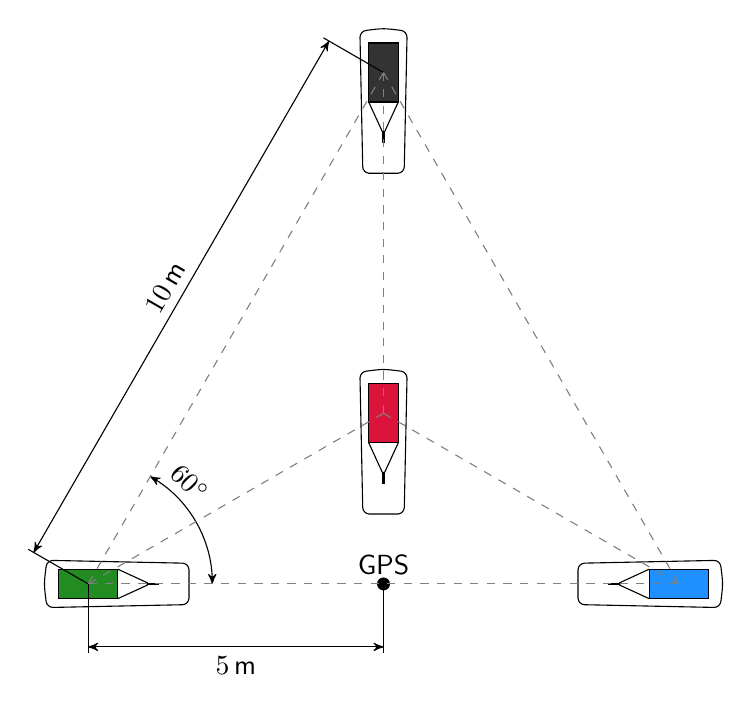
\begin{tikzpicture}
    [font=\sffamily, x=.75cm, y=.75cm,
     >=stealth',
%     thick,
    ]
    \foreach \sc / \col / \sx / \sy / \angle [count=\si] in
             {A/black!80!white/0/8.66/0, B/Crimson/0/2.89/0,
              C/ForestGreen/-5/0/90, D/DodgerBlue/5/0/-90} {
        \coordinate (\sc) at (\sx, \sy);
        \begin{scope}[shift={(\sc)}, rotate=\angle]
            % Skibox
            \draw[fill=white, rounded corners=2.25pt]
                (-.4, .7) .. controls (0, .75) ..  (.4, .7) --
                (.35, -1.7) .. controls (0, -1.72) ..  (-.35, -1.7) --
                cycle;
            % Scintillator
            \draw[fill=\col] (-.25, .5) rectangle (.25, -.5);
            % Lightguide
            \draw (-.25, -.5) -- (-.02, -1) --(.02, -1) -- (.25, -.5);
            % PMT
            \fill (-.02, -1) rectangle (.02, -1.2);
            % Detector number
            %\node[color=gray] at (-.75, 1) {\Large \si};
        \end{scope}
    }

    \coordinate (G) at (0, 0);
    % GPS
    \draw[fill] (G) circle (.10) node [above] {GPS};

    % Create coordinates for drawing distance lines
    \foreach \sc in {A,...,D,G} {
        \foreach \ssc in {A,...,D,G} {
            % Create both in and outside coordinates
            \coordinate (\sc'\ssc) at ($ (\sc)!.8cm!90:(\ssc) $);
            \coordinate (\sc''\ssc) at ($ (\sc)!.8cm!-90:(\ssc) $);
        }
    }

    \draw (A) -- ($ (A)!1.1!(A''C) $);
    \draw (C) -- ($ (C)!1.1!(C'A) $);
    \draw[<->] (A''C) -- (C'A) node [midway, above, sloped] {\SI{10}{\meter}};

    \draw (C) -- ($ (C)!1.1!(C''G) $);
    \draw (G) -- ($ (G)!1.1!(G'C) $);
    \draw[<->] (C''G) -- (G'C) node [midway, below] {\SI{5}{\meter}};

    \draw[<->] (C) ++(0:2.1) arc (0:60:2.1)
        node[near end, above, sloped] {\SI{60}{\degree}};

    \draw[dashed,gray] (A) -- (B);
    \draw[dashed,gray] (A) -- (C);
    \draw[dashed,gray] (A) -- (D);
    \draw[dashed,gray] (B) -- (C);
    \draw[dashed,gray] (B) -- (D);
    \draw[dashed,gray] (C) -- (D);
\end{tikzpicture}

\end{document}
